%%%%%%%%%%%%%%%%%%%%%%%%%%%%%%%%%%%%%%%%%%%%%%%%%%%%%%%%%%%%%%%%%%%%%%%%%%
% Conference poster -- Utah AI Convergence
%
% A0 landscape "better poster" (MIT-improved BetterPoster layout): a large
% central billboard with one plain-language takeaway, flanked by a short
% left column (the challenge) and a right column (what we did / what we
% learned), with a bottom strip for conclusions, future work, and links.
%
% Standalone, separate from the journal manuscript (paper/main.tex). It is
% deliberately jargon-free and frames the prototype as a CASE STUDY of
% generative-AI hardware design. Every claim and image is REAL, completed
% work: shaded CAD renders are the actual parts/assemblies from the public
% repository's design branches; no synthetic dispensing data, performance
% numbers, or placeholder figures appear here.
%%%%%%%%%%%%%%%%%%%%%%%%%%%%%%%%%%%%%%%%%%%%%%%%%%%%%%%%%%%%%%%%%%%%%%%%%%%

\documentclass[a0,landscape]{a0poster}

\usepackage[utf8]{inputenc}
\usepackage[T1]{fontenc}
\usepackage{helvet}
\renewcommand{\familydefault}{\sfdefault}
\usepackage{graphicx}
\usepackage{tikz}
\usepackage[most]{tcolorbox}
\usepackage{qrcode}
\usepackage{ragged2e}
\usepackage{microtype}

\graphicspath{{assets/}}

% ---- palette ---------------------------------------------------------
\definecolor{navy}{RGB}{18,46,82}
\definecolor{steel}{RGB}{52,96,148}
\definecolor{ember}{RGB}{196,76,40}
\definecolor{panelbg}{RGB}{238,242,247}
\definecolor{rule}{RGB}{210,218,228}

\setlength{\parindent}{0pt}
\setlength{\parskip}{0.5em}
\pagestyle{empty}

% ---- reusable section panel -----------------------------------------
\newtcolorbox{panel}[1]{
  enhanced, breakable=false,
  colback=panelbg, colframe=steel,
  boxrule=0pt, leftrule=10pt,
  arc=6pt, outer arc=6pt,
  left=18pt, right=18pt, top=14pt, bottom=16pt,
  fonttitle=\bfseries\LARGE\color{navy},
  coltitle=navy,
  title={#1},
  attach title to upper=\par\vspace{8pt},
}

% ---- a "finding" mini-box with a heading ----------------------------
\newcommand{\finding}[2]{%
  {\color{ember}\bfseries\Large #1}\\[2pt]#2\par\vspace{6pt}}

% ---- key-stat tile --------------------------------------------------
\newcommand{\stat}[2]{%
  \begin{minipage}[t]{0.30\linewidth}\centering
    {\color{navy}\Huge\bfseries #1}\\[6pt]
    {\large #2}
  \end{minipage}}

\begin{document}

%======================================================================
% TITLE BAND
%======================================================================
\begin{tcolorbox}[enhanced, colback=navy, colframe=navy, arc=8pt,
  left=30pt, right=30pt, top=16pt, bottom=16pt, boxrule=0pt]
\color{white}
\begin{minipage}[c]{0.80\linewidth}
  \raggedright
  {\veryHuge\bfseries We built a working lab instrument\\[10pt]
   without CAD software---generative AI designed every part}\\[18pt]
  {\Large Sam Charles \quad Will Mulberry \quad Luke Winters \quad
   Carl Robison \quad Gage Erickson \quad Sterling G. Baird}\\[6pt]
  {\large Brigham Young University \ \textbar\ University of Utah
   \qquad\textbullet\qquad Utah AI Convergence}
\end{minipage}\hfill
\begin{minipage}[c]{0.16\linewidth}\centering
  \colorbox{white}{\makebox[5cm][c]{\raisebox{0pt}{%
    \color{black}\qrcode[height=4.4cm]{https://github.com/vertical-cloud-lab/powder-doser}}}}\\[8pt]
  {\large Open repository\\ \& full design history}
\end{minipage}
\end{tcolorbox}

\vspace{10pt}

%======================================================================
% THREE-COLUMN BODY
%======================================================================
\noindent
%---------------------------------------------------------------- LEFT
\begin{minipage}[t]{0.275\linewidth}
\Large
\begin{panel}{The challenge}
  Self-driving laboratories let robots run experiments and let software
  decide what to try next. They handle \textbf{liquids} well, but most
  still weigh out \textbf{powders by hand}.

  Machines that dose powders automatically exist, but they cost
  \textbf{tens to hundreds of thousands of dollars}, putting them out of
  reach for most academic labs.
\end{panel}

\vspace{14pt}
\begin{panel}{Our question}
  Generative AI can already write code and produce 3D shapes. We asked a
  practical question:

  \textbf{Can today's AI design a real, working physical instrument from
  start to finish}---if a small human team sets the goals and checks the
  work?

  To make the test honest, we set one strict rule.
\end{panel}

\vspace{14pt}
\begin{tcolorbox}[enhanced, colback=ember, colframe=ember, arc=6pt,
  left=18pt,right=18pt,top=14pt,bottom=14pt, boxrule=0pt]
  \color{white}\centering
  {\Large\bfseries The rule}\\[8pt]
  {\huge\bfseries No conventional CAD software\\(SolidWorks, Fusion 360)
  was used at any point.}
\end{tcolorbox}
\end{minipage}
\hfill
%-------------------------------------------------------------- CENTER
\begin{minipage}[t]{0.385\linewidth}
\centering
\begin{tcolorbox}[enhanced, colback=white, colframe=navy, arc=8pt,
  left=20pt, right=20pt, top=14pt, bottom=14pt, boxrule=4pt]
  \color{navy}
  {\huge\bfseries\justifying
   Generative AI designed every part of a real, working laboratory
   instrument---and the complete, honest design history, including its
   failures, is public.}
\end{tcolorbox}

\vspace{14pt}
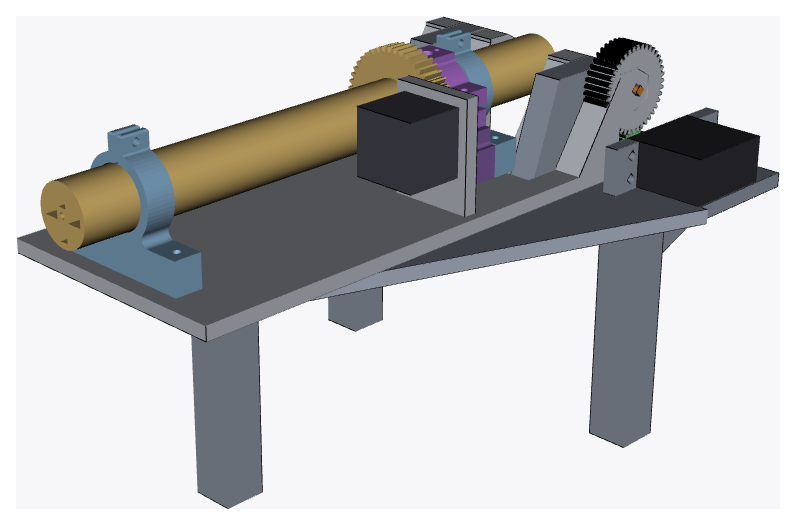
\includegraphics[width=0.66\linewidth]{assembly_iso_final.png}\\[6pt]
{\large The single-channel powder doser. Humans chose the design and
 reviewed, printed, and tested every part; AI tools created all of the
 3D models.}

\vspace{16pt}
\hrule height 2pt
\vspace{14pt}
\stat{97}{logged design iterations, including every failure}\hfill
\stat{0}{uses of conventional CAD software}\hfill
\stat{<\$200}{in parts; a \$6 microcontroller runs it}

\vspace{14pt}
\hrule height 2pt
\end{minipage}
\hfill
%--------------------------------------------------------------- RIGHT
\begin{minipage}[t]{0.305\linewidth}
\Large
\begin{panel}{What we did}
  We worked in \textbf{two AI ways}:
  \vspace{4pt}

  \textbf{1. Programmatic CAD.} AI ``coding agents'' wrote each part as
  computer code; the code became a 3D model and a picture automatically,
  and our team reviewed every result and asked for fixes.

  \textbf{2. Chat-driven design.} Later we used Zoo Design Studio and its
  AI agent, Zookeeper, driven almost entirely by typing instructions in
  plain language rather than by drawing.
\end{panel}

\vspace{12pt}
\begin{panel}{What we learned}
  \finding{Part by part beats all at once.}{Asking the AI for the whole
  machine gave parts that overlapped or floated with no room for motors.
  Asking for \emph{one part at a time}, with clear instructions on how it
  connects to its neighbours, worked.}

  \finding{The AI needs constant checking.}{It would quietly change parts
  we had already finished, so every new version had to be re-inspected.
  Automated checks plus human review caught the problems.}

  \finding{Honest about the trade-off.}{An expert in normal CAD would have
  been faster and cleaner. What AI bought instead was a complete written
  record of every decision, prompt, and mistake---making the whole project
  reproducible.}
\end{panel}

\vspace{12pt}
\begin{minipage}[t]{0.485\linewidth}\centering
  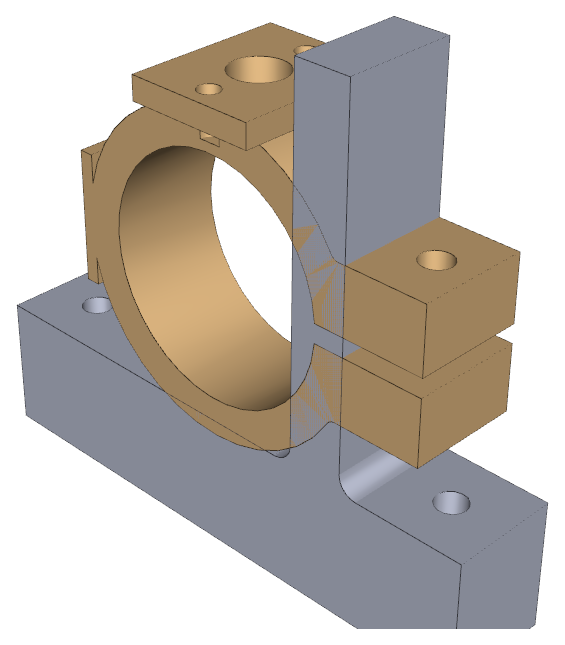
\includegraphics[height=8cm]{tap_collar_v1_iso.png}\\[4pt]
  {\normalsize\color{ember}\bfseries First AI attempt:}\\
  {\normalsize impossible to build}
\end{minipage}\hfill
\begin{minipage}[t]{0.485\linewidth}\centering
  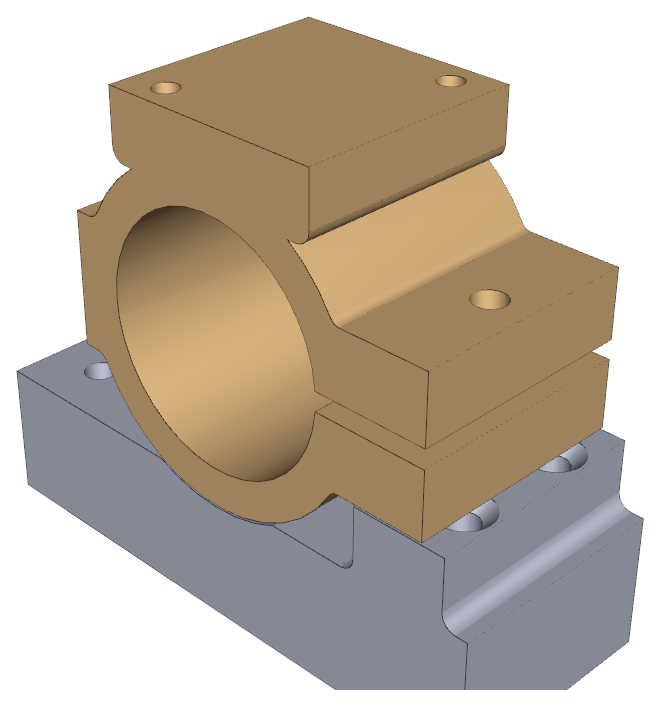
\includegraphics[height=8cm]{tap_collar_final_iso.png}\\[4pt]
  {\normalsize\color{steel}\bfseries After review:}\\
  {\normalsize a part that prints and works}
\end{minipage}
\end{minipage}

\vspace{10pt}

%======================================================================
% BOTTOM STRIP
%======================================================================
\noindent
\begin{tcolorbox}[enhanced, colback=panelbg, colframe=navy, arc=8pt,
  left=28pt, right=28pt, top=18pt, bottom=18pt, boxrule=0pt]
\Large
\begin{minipage}[t]{0.62\linewidth}
  {\LARGE\bfseries\color{navy} Conclusion \& what's next}\\[8pt]
  We designed and built a real laboratory instrument \textbf{entirely with
  generative AI, under human direction, and without ever opening
  conventional CAD software}. Because the full project history---every
  prompt, every generated part, and every failure---is public, the build
  doubles as a case study of what AI can and cannot yet do in hardware
  design. We have early CAD for a multi-powder version and continue to
  test new AI design tools.
\end{minipage}\hfill
\begin{minipage}[t]{0.33\linewidth}
  {\LARGE\bfseries\color{navy} Everything is open}\\[8pt]
  Design files, firmware, and the complete log of AI prompts and
  responses are freely available:\\[8pt]
  {\large\texttt{github.com/vertical-cloud-lab/\\powder-doser}}
\end{minipage}
\end{tcolorbox}

\end{document}
